\documentclass[11pt,landscape]{article}
\usepackage[margin=8mm]{geometry}
\usepackage[T1]{fontenc}
\usepackage[utf8]{inputenc}
\usepackage{lmodern}
\usepackage{amsmath}
\usepackage{tikz}
\usetikzlibrary{arrows.meta, positioning, fit, backgrounds, calc}
\pagestyle{empty}

\begin{document}

\begin{center}
\Large GRLNet: Temporal Unrolling View
\end{center}

\vspace{2mm}

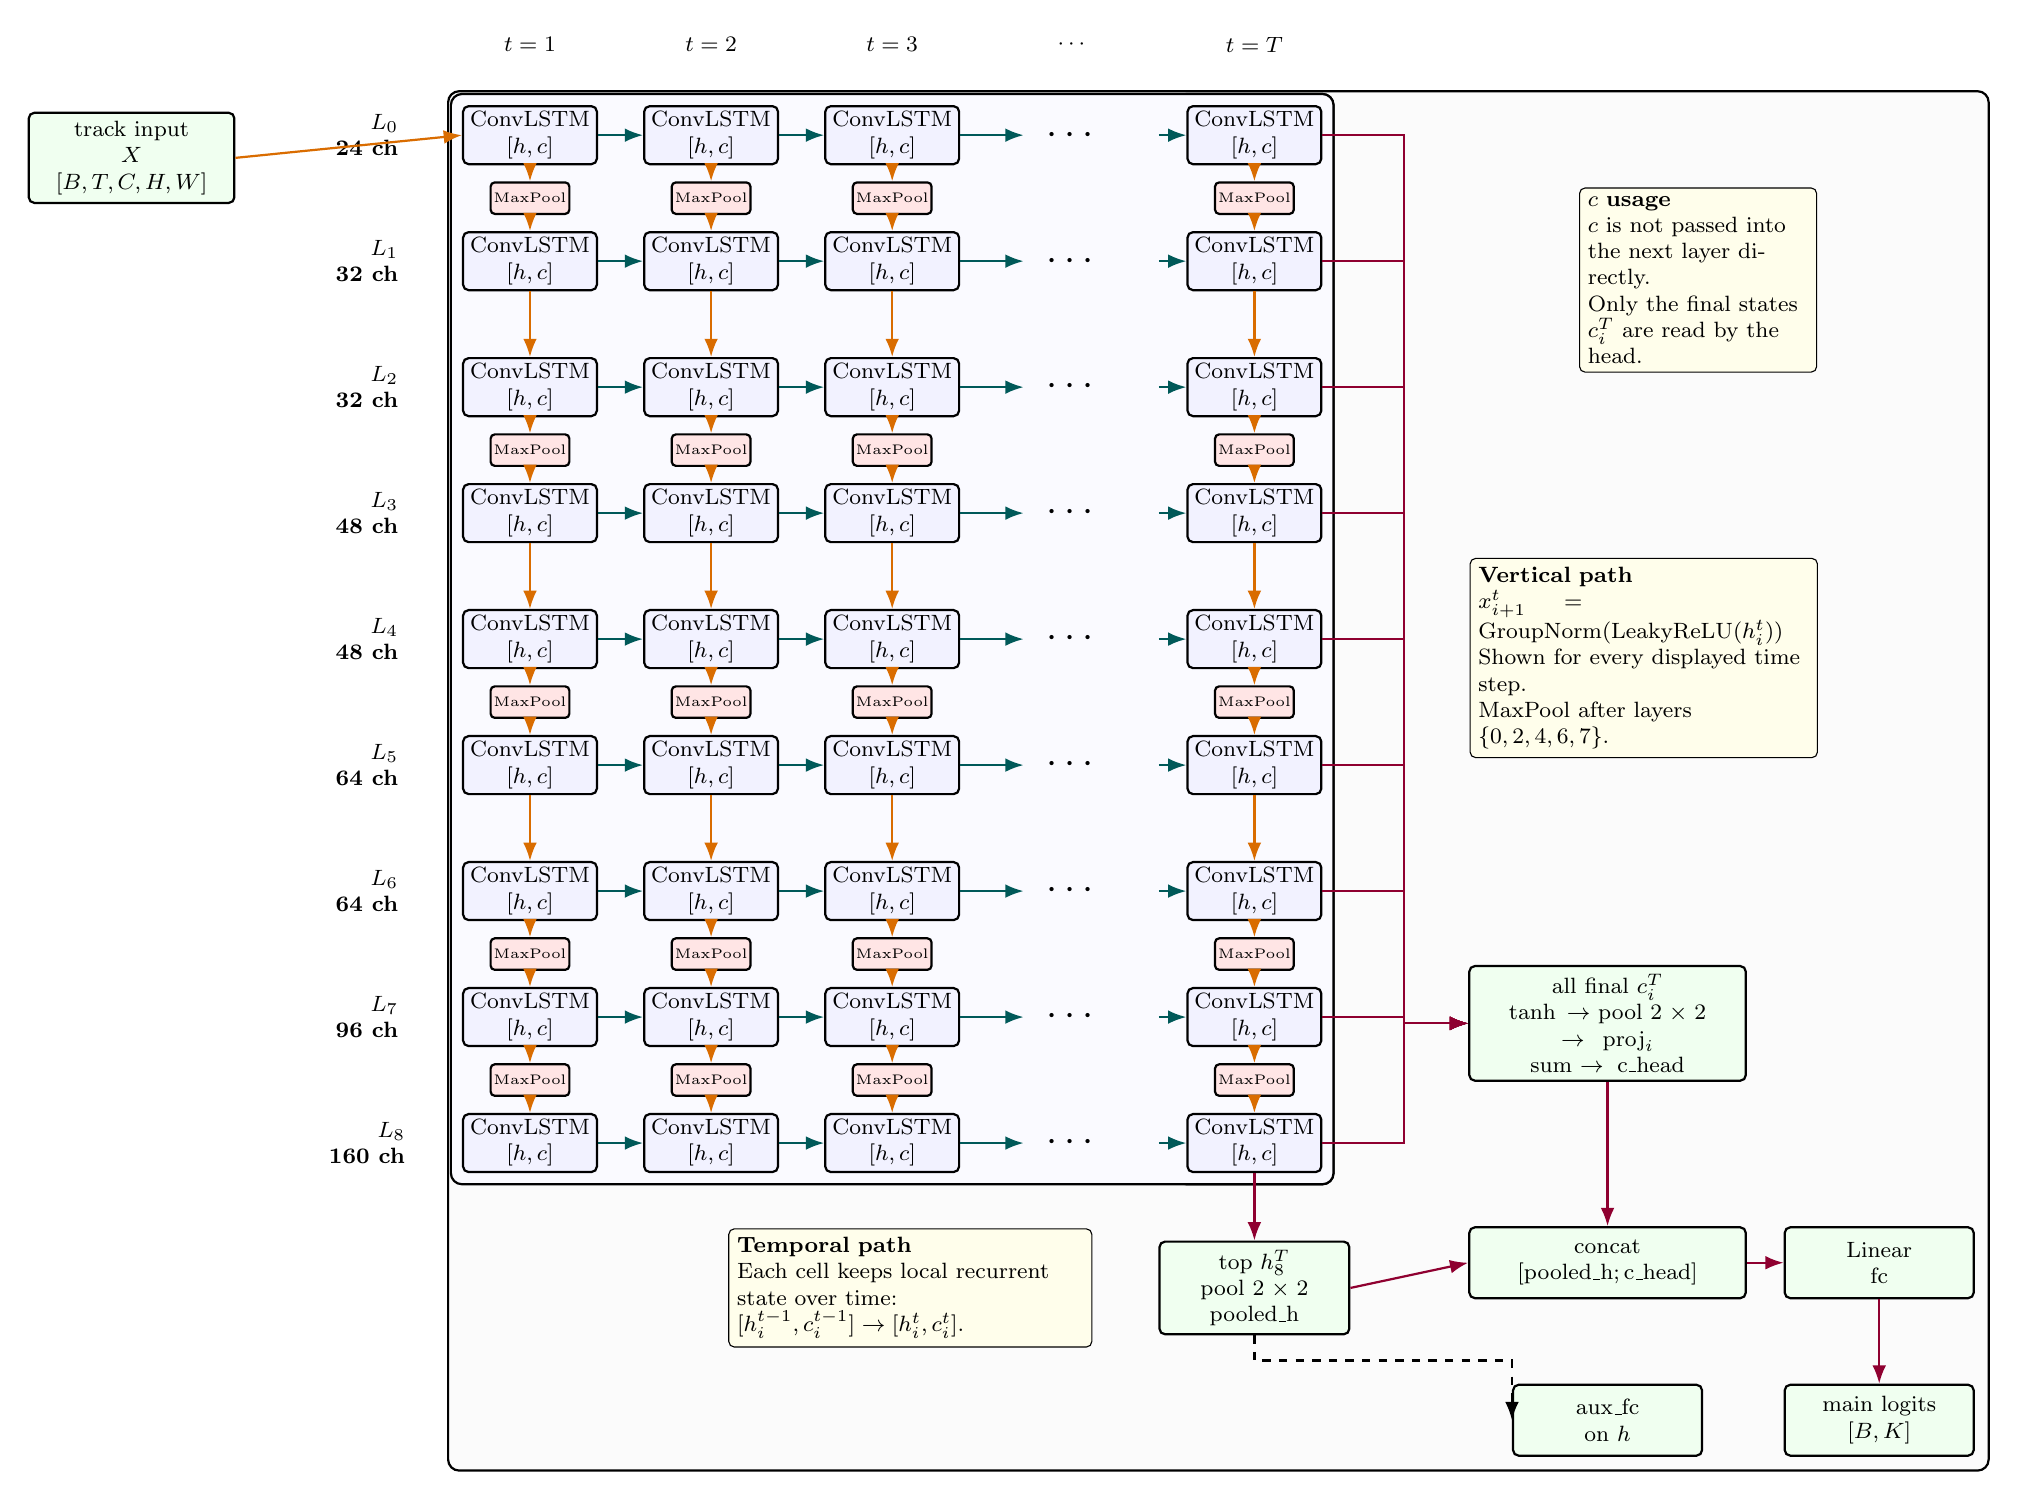
\begin{tikzpicture}[
    >=Latex,
    x=23mm,
    y=16mm,
    cell/.style={draw, rounded corners=2pt, thick, align=center, inner sep=2pt, minimum width=17mm, minimum height=7mm, fill=blue!5, font=\footnotesize},
    vpool/.style={draw, rounded corners=1.5pt, thick, align=center, inner sep=1pt, minimum width=10mm, minimum height=4mm, fill=red!10, font=\tiny},
    head/.style={draw, rounded corners=2pt, thick, align=center, inner sep=3pt, minimum width=24mm, minimum height=9mm, fill=green!6, font=\footnotesize},
    note/.style={draw, rounded corners=2pt, align=left, inner sep=3pt, fill=yellow!8, font=\footnotesize},
    timelabel/.style={font=\footnotesize\bfseries},
    layerlabel/.style={font=\footnotesize\bfseries, align=right},
    recur/.style={->, thick, teal!70!black},
    up/.style={->, thick, orange!85!black},
    readout/.style={->, thick, purple!75!black},
    aux/.style={->, thick, dashed}
]

% time labels
\node[timelabel] at (0,0.72) {$t=1$};
\node[timelabel] at (1,0.72) {$t=2$};
\node[timelabel] at (2,0.72) {$t=3$};
\node[timelabel] at (3,0.72) {$\cdots$};
\node[timelabel] at (4,0.72) {$t=T$};

% layer labels
\node[layerlabel] at (-0.9,0) {$L_0$\\24 ch};
\node[layerlabel] at (-0.9,-1) {$L_1$\\32 ch};
\node[layerlabel] at (-0.9,-2) {$L_2$\\32 ch};
\node[layerlabel] at (-0.9,-3) {$L_3$\\48 ch};
\node[layerlabel] at (-0.9,-4) {$L_4$\\48 ch};
\node[layerlabel] at (-0.9,-5) {$L_5$\\64 ch};
\node[layerlabel] at (-0.9,-6) {$L_6$\\64 ch};
\node[layerlabel] at (-0.9,-7) {$L_7$\\96 ch};
\node[layerlabel] at (-0.9,-8) {$L_8$\\160 ch};

% grid cells
\node[cell] (lzeroone)   at (0,0)  {ConvLSTM\\$[h,c]$};
\node[cell] (lzerotwo)   at (1,0)  {ConvLSTM\\$[h,c]$};
\node[cell] (lzerothree) at (2,0)  {ConvLSTM\\$[h,c]$};
\node[cell] (lzeroT)     at (4,0)  {ConvLSTM\\$[h,c]$};

\node[cell] (loneone)    at (0,-1) {ConvLSTM\\$[h,c]$};
\node[cell] (lonetwo)    at (1,-1) {ConvLSTM\\$[h,c]$};
\node[cell] (lonethree)  at (2,-1) {ConvLSTM\\$[h,c]$};
\node[cell] (loneT)      at (4,-1) {ConvLSTM\\$[h,c]$};

\node[cell] (ltwoone)    at (0,-2) {ConvLSTM\\$[h,c]$};
\node[cell] (ltwotwo)    at (1,-2) {ConvLSTM\\$[h,c]$};
\node[cell] (ltwothree)  at (2,-2) {ConvLSTM\\$[h,c]$};
\node[cell] (ltwoT)      at (4,-2) {ConvLSTM\\$[h,c]$};

\node[cell] (lthreeone)   at (0,-3) {ConvLSTM\\$[h,c]$};
\node[cell] (lthreetwo)   at (1,-3) {ConvLSTM\\$[h,c]$};
\node[cell] (lthreethree) at (2,-3) {ConvLSTM\\$[h,c]$};
\node[cell] (lthreeT)     at (4,-3) {ConvLSTM\\$[h,c]$};

\node[cell] (lfourone)   at (0,-4) {ConvLSTM\\$[h,c]$};
\node[cell] (lfourtwo)   at (1,-4) {ConvLSTM\\$[h,c]$};
\node[cell] (lfourthree) at (2,-4) {ConvLSTM\\$[h,c]$};
\node[cell] (lfourT)     at (4,-4) {ConvLSTM\\$[h,c]$};

\node[cell] (lfiveone)   at (0,-5) {ConvLSTM\\$[h,c]$};
\node[cell] (lfivetwo)   at (1,-5) {ConvLSTM\\$[h,c]$};
\node[cell] (lfivethree) at (2,-5) {ConvLSTM\\$[h,c]$};
\node[cell] (lfiveT)     at (4,-5) {ConvLSTM\\$[h,c]$};

\node[cell] (lsixone)   at (0,-6) {ConvLSTM\\$[h,c]$};
\node[cell] (lsixtwo)   at (1,-6) {ConvLSTM\\$[h,c]$};
\node[cell] (lsixthree) at (2,-6) {ConvLSTM\\$[h,c]$};
\node[cell] (lsixT)     at (4,-6) {ConvLSTM\\$[h,c]$};

\node[cell] (lsevenone)   at (0,-7) {ConvLSTM\\$[h,c]$};
\node[cell] (lseventwo)   at (1,-7) {ConvLSTM\\$[h,c]$};
\node[cell] (seventhree)  at (2,-7) {ConvLSTM\\$[h,c]$};
\node[cell] (lsevenT)     at (4,-7) {ConvLSTM\\$[h,c]$};

\node[cell] (leightone)   at (0,-8) {ConvLSTM\\$[h,c]$};
\node[cell] (leighttwo)   at (1,-8) {ConvLSTM\\$[h,c]$};
\node[cell] (leightthree) at (2,-8) {ConvLSTM\\$[h,c]$};
\node[cell] (leightT)     at (4,-8) {ConvLSTM\\$[h,c]$};

% ellipsis column
\foreach \r in {0,...,8} {
    \node at (3,-\r) {\Large$\cdots$};
}

% vertical pooling markers after layers {0,2,4,6,7}
\node[vpool] (p01) at (0,-0.5) {MaxPool};
\node[vpool] (p02) at (1,-0.5) {MaxPool};
\node[vpool] (p03) at (2,-0.5) {MaxPool};
\node[vpool] (p0T) at (4,-0.5) {MaxPool};

\node[vpool] (p21) at (0,-2.5) {MaxPool};
\node[vpool] (p22) at (1,-2.5) {MaxPool};
\node[vpool] (p23) at (2,-2.5) {MaxPool};
\node[vpool] (p2T) at (4,-2.5) {MaxPool};

\node[vpool] (p41) at (0,-4.5) {MaxPool};
\node[vpool] (p42) at (1,-4.5) {MaxPool};
\node[vpool] (p43) at (2,-4.5) {MaxPool};
\node[vpool] (p4T) at (4,-4.5) {MaxPool};

\node[vpool] (p61) at (0,-6.5) {MaxPool};
\node[vpool] (p62) at (1,-6.5) {MaxPool};
\node[vpool] (p63) at (2,-6.5) {MaxPool};
\node[vpool] (p6T) at (4,-6.5) {MaxPool};

\node[vpool] (p71) at (0,-7.5) {MaxPool};
\node[vpool] (p72) at (1,-7.5) {MaxPool};
\node[vpool] (p73) at (2,-7.5) {MaxPool};
\node[vpool] (p7T) at (4,-7.5) {MaxPool};

% input
\node[head, text width=24mm] (input) at (-2.2,-0.18) {track input\\$X$\\$[B,T,C,H,W]$};
\draw[up] (input.east) -- (lzeroone.west);

% recurrent arrows
\draw[recur] (lzeroone.east) -- (lzerotwo.west);
\draw[recur] (lzerotwo.east) -- (lzerothree.west);
\draw[recur] (lzerothree.east) -- ++(0.35,0);
\draw[recur] ([xshift=-0.35cm]lzeroT.west) -- (lzeroT.west);

\draw[recur] (loneone.east) -- (lonetwo.west);
\draw[recur] (lonetwo.east) -- (lonethree.west);
\draw[recur] (lonethree.east) -- ++(0.35,0);
\draw[recur] ([xshift=-0.35cm]loneT.west) -- (loneT.west);

\draw[recur] (ltwoone.east) -- (ltwotwo.west);
\draw[recur] (ltwotwo.east) -- (ltwothree.west);
\draw[recur] (ltwothree.east) -- ++(0.35,0);
\draw[recur] ([xshift=-0.35cm]ltwoT.west) -- (ltwoT.west);

\draw[recur] (lthreeone.east) -- (lthreetwo.west);
\draw[recur] (lthreetwo.east) -- (lthreethree.west);
\draw[recur] (lthreethree.east) -- ++(0.35,0);
\draw[recur] ([xshift=-0.35cm]lthreeT.west) -- (lthreeT.west);

\draw[recur] (lfourone.east) -- (lfourtwo.west);
\draw[recur] (lfourtwo.east) -- (lfourthree.west);
\draw[recur] (lfourthree.east) -- ++(0.35,0);
\draw[recur] ([xshift=-0.35cm]lfourT.west) -- (lfourT.west);

\draw[recur] (lfiveone.east) -- (lfivetwo.west);
\draw[recur] (lfivetwo.east) -- (lfivethree.west);
\draw[recur] (lfivethree.east) -- ++(0.35,0);
\draw[recur] ([xshift=-0.35cm]lfiveT.west) -- (lfiveT.west);

\draw[recur] (lsixone.east) -- (lsixtwo.west);
\draw[recur] (lsixtwo.east) -- (lsixthree.west);
\draw[recur] (lsixthree.east) -- ++(0.35,0);
\draw[recur] ([xshift=-0.35cm]lsixT.west) -- (lsixT.west);

\draw[recur] (lsevenone.east) -- (lseventwo.west);
\draw[recur] (lseventwo.east) -- (seventhree.west);
\draw[recur] (seventhree.east) -- ++(0.35,0);
\draw[recur] ([xshift=-0.35cm]lsevenT.west) -- (lsevenT.west);

\draw[recur] (leightone.east) -- (leighttwo.west);
\draw[recur] (leighttwo.east) -- (leightthree.west);
\draw[recur] (leightthree.east) -- ++(0.35,0);
\draw[recur] ([xshift=-0.35cm]leightT.west) -- (leightT.west);

% upward arrows between layers at each shown time step
\draw[up] (lzeroone.south) -- (p01.north);
\draw[up] (p01.south) -- (loneone.north);
\draw[up] (loneone.south) -- (ltwoone.north);
\draw[up] (ltwoone.south) -- (p21.north);
\draw[up] (p21.south) -- (lthreeone.north);
\draw[up] (lthreeone.south) -- (lfourone.north);
\draw[up] (lfourone.south) -- (p41.north);
\draw[up] (p41.south) -- (lfiveone.north);
\draw[up] (lfiveone.south) -- (lsixone.north);
\draw[up] (lsixone.south) -- (p61.north);
\draw[up] (p61.south) -- (lsevenone.north);
\draw[up] (lsevenone.south) -- (p71.north);
\draw[up] (p71.south) -- (leightone.north);

\draw[up] (lzerotwo.south) -- (p02.north);
\draw[up] (p02.south) -- (lonetwo.north);
\draw[up] (lonetwo.south) -- (ltwotwo.north);
\draw[up] (ltwotwo.south) -- (p22.north);
\draw[up] (p22.south) -- (lthreetwo.north);
\draw[up] (lthreetwo.south) -- (lfourtwo.north);
\draw[up] (lfourtwo.south) -- (p42.north);
\draw[up] (p42.south) -- (lfivetwo.north);
\draw[up] (lfivetwo.south) -- (lsixtwo.north);
\draw[up] (lsixtwo.south) -- (p62.north);
\draw[up] (p62.south) -- (lseventwo.north);
\draw[up] (lseventwo.south) -- (p72.north);
\draw[up] (p72.south) -- (leighttwo.north);

\draw[up] (lzerothree.south) -- (p03.north);
\draw[up] (p03.south) -- (lonethree.north);
\draw[up] (lonethree.south) -- (ltwothree.north);
\draw[up] (ltwothree.south) -- (p23.north);
\draw[up] (p23.south) -- (lthreethree.north);
\draw[up] (lthreethree.south) -- (lfourthree.north);
\draw[up] (lfourthree.south) -- (p43.north);
\draw[up] (p43.south) -- (lfivethree.north);
\draw[up] (lfivethree.south) -- (lsixthree.north);
\draw[up] (lsixthree.south) -- (p63.north);
\draw[up] (p63.south) -- (seventhree.north);
\draw[up] (seventhree.south) -- (p73.north);
\draw[up] (p73.south) -- (leightthree.north);

\draw[up] (lzeroT.south) -- (p0T.north);
\draw[up] (p0T.south) -- (loneT.north);
\draw[up] (loneT.south) -- (ltwoT.north);
\draw[up] (ltwoT.south) -- (p2T.north);
\draw[up] (p2T.south) -- (lthreeT.north);
\draw[up] (lthreeT.south) -- (lfourT.north);
\draw[up] (lfourT.south) -- (p4T.north);
\draw[up] (p4T.south) -- (lfiveT.north);
\draw[up] (lfiveT.south) -- (lsixT.north);
\draw[up] (lsixT.south) -- (p6T.north);
\draw[up] (p6T.south) -- (lsevenT.north);
\draw[up] (lsevenT.south) -- (p7T.north);
\draw[up] (p7T.south) -- (leightT.north);

% notes
\node[note, text width=42mm] (upnote) at (6.15,-4.15) {
\textbf{Vertical path}\\
$x_{i+1}^{t}=\mathrm{GroupNorm}(\mathrm{LeakyReLU}(h_i^t))$\\
Shown for every displayed time step.\\
MaxPool after layers $\{0,2,4,6,7\}$.
};

\node[note, text width=44mm] (recur_note) at (2.1,-9.15) {
\textbf{Temporal path}\\
Each cell keeps local recurrent state over time:\\
$[h_i^{t-1}, c_i^{t-1}] \rightarrow [h_i^t, c_i^t]$.
};

% heads
\node[head, text width=22mm] (hhead) at (4.0,-9.15) {
top $h_8^T$\\
pool $2\times2$\\
$\mathrm{pooled\_h}$
};

\node[head, text width=33mm] (chead) at (5.95,-7.05) {
all final $c_i^T$\\
$\tanh \rightarrow$ pool $2\times2$\\
$\rightarrow \mathrm{proj}_i$\\
sum $\rightarrow \mathrm{c\_head}$
};

\node[head, text width=33mm] (concat) at (5.95,-8.95) {
concat\\
$[\mathrm{pooled\_h};\mathrm{c\_head}]$
};

\node[head, text width=16mm] (fc) at (7.45,-8.95) {
Linear\\
fc
};

\node[head, text width=18mm] (out) at (7.45,-10.2) {
main logits\\
$[B,K]$
};

\node[head, text width=16mm] (auxhead) at (5.95,-10.2) {
aux\_fc\\
on $h$
};

% readout arrows
\draw[readout] (leightT.south) -- (hhead.north);
\draw[readout] (lzeroT.east) -- ++(0.45,0) |- (chead.west);
\draw[readout] (loneT.east) -- ++(0.45,0) |- (chead.west);
\draw[readout] (ltwoT.east) -- ++(0.45,0) |- (chead.west);
\draw[readout] (lthreeT.east) -- ++(0.45,0) |- (chead.west);
\draw[readout] (lfourT.east) -- ++(0.45,0) |- (chead.west);
\draw[readout] (lfiveT.east) -- ++(0.45,0) |- (chead.west);
\draw[readout] (lsixT.east) -- ++(0.45,0) |- (chead.west);
\draw[readout] (lsevenT.east) -- ++(0.45,0) |- (chead.west);
\draw[readout] (leightT.east) -- ++(0.45,0) |- (chead.west);
\draw[readout] (hhead.east) -- (concat.west);
\draw[readout] (chead.south) -- (concat.north);
\draw[readout] (concat.east) -- (fc.west);
\draw[readout] (fc.south) -- (out.north);
\draw[aux] (hhead.south) -- ++(0,-0.2) -| (auxhead.west);

\node[note, text width=28mm] (chead_note) at (6.45,-1.15) {
\textbf{$c$ usage}\\
$c$ is not passed into the next layer directly.\\
Only the final states $c_i^T$ are read by the head.
};

\begin{scope}[on background layer]
    \node[draw, rounded corners=4pt, thick, fit=(lzeroone)(leightT)(upnote)(recur_note)(hhead)(chead)(concat)(fc)(out)(auxhead)(chead_note), inner sep=5pt, fill=gray!3] {};
    \node[draw, rounded corners=4pt, thick, fit=(lzeroT)(leightT), inner sep=4pt, fill=orange!4] {};
    \node[draw, rounded corners=4pt, thick, fit=(lzeroone)(leightT), inner sep=4pt, fill=blue!2] {};
\end{scope}

\end{tikzpicture}

\end{document}
